\documentclass[UTF8,fontset=none,12pt]{ctexart}

\setCJKmainfont{Songti SC}
\setCJKsansfont{PingFang SC}
\setCJKmonofont{Songti SC}

\usepackage[a4paper,margin=2.35cm]{geometry}
\usepackage{amsmath,amssymb,amsthm,mathtools,bm}
\usepackage{graphicx}
\usepackage{float}
\usepackage{booktabs}
\usepackage{array}
\usepackage{enumitem}
\usepackage[hidelinks]{hyperref}

\title{数值线性代数\quad 第 31 讲：奇异值分解的计算}
\author{Lloyd N. Trefethen、David Bau III\quad 中文阅读版}
\date{}

\begin{document}
\maketitle
\pagestyle{plain}

任意矩阵的奇异值分解（SVD）可以归结为一个 Hermitian 方阵的特征值分解，
但最直接的做法并不稳定。标准的 SVD 算法隐式地采用了另一种约化到 Hermitian
形式的方法。为了提高速度，矩阵首先通过左右酉变换约化为双对角形式。

\section*{A 的 SVD 与 $A^*A$ 的特征值}

如定理 5.4 所述，对于 $m\times n$ 矩阵 $A$（$m\ge n$），若
\[
A=U\Sigma V^*,
\]
则它的 SVD 与矩阵 $A^*A$ 的特征值分解有关：

\[
A^*A=V\Sigma^*\Sigma V^*.
\]

因此，从数学上看，我们可以按下面的步骤计算 $A$ 的 SVD：

\begin{enumerate}[label=\arabic*.]
\item 构造 $A^*A$；
\item 计算特征值分解 $A^*A=V\Lambda V^*$；
\item 取 $\Sigma$ 为 $\Lambda$ 的非负对角平方根，并将其视为 $m\times n$ 矩形对角矩阵；
\item 求解矩阵方程 $U\Sigma=AV$，得到酉矩阵 $U$（例如通过 QR 分解）。
\end{enumerate}

这个算法经常被使用，甚至有人在独立重新发现 SVD 时也会采用它。矩阵
$A^*A$ 称为 $A$ 的协方差矩阵，在统计学和其他领域中有熟悉的解释。然而，该
算法并不稳定，因为它把 SVD 问题约化成了一个可能对扰动更加敏感的特征值问题。

困难可以这样说明。我们已经知道，当 Hermitian 矩阵 $A^*A$ 被扰动
$\delta B$ 后，每个特征值的绝对变化量不超过扰动的 2-范数。由习题 26.3(b)，

$$
|\lambda_k(A^*A+\delta B)-\lambda_k(A^*A)|
\le \|\delta B\|_2.
$$

另一方面，如下式 (31.2) 所暗示的，$A$ 的奇异值满足类似的界：

$$
|\sigma_k(A+\delta A)-\sigma_k(A)|\le \|\delta A\|_2.
$$

因此，一个后向稳定的奇异值算法会得到满足

\begin{equation}
\widetilde\sigma_k=\sigma_k(A+\delta A),
\qquad
\frac{\|\delta A\|}{\|A\|}=O(\varepsilon_{\mathrm{machine}}),
\tag{31.1}
\end{equation}

的 $\widetilde\sigma_k$，从而有

$$
|\widetilde\sigma_k-\sigma_k|
=O(\varepsilon_{\mathrm{machine}}\|A\|).
$$

现在观察通过计算 $\lambda_k(A^*A)$ 来求奇异值时会发生什么。即使
$\lambda_k(A^*A)$ 被稳定地计算出来，我们也只能期待

$$
|\widetilde\lambda_k-\lambda_k|
=O(\varepsilon_{\mathrm{machine}}\|A^*A\|)
=O(\varepsilon_{\mathrm{machine}}\|A\|^2).
$$

开平方得到 $\sigma_k$ 时，

$$
|\widetilde\sigma_k-\sigma_k|
=O\!\left(\frac{|\widetilde\lambda_k-\lambda_k|}
{\sqrt{\widetilde\lambda_k}}\right)
=O\!\left(\frac{\varepsilon_{\mathrm{machine}}\|A\|^2}{\sigma_k}\right).
$$

与前面的结果相比，这多了一个 $O(\|A\|/\sigma_k)$ 的因子。当
$\sigma_k\approx\|A\|$，即对于最大的奇异值来说，这不是问题；但对于满足
$\sigma_k\ll\|A\|$ 的奇异值，它会造成严重影响。对于最小奇异值 $\sigma_n$，
我们必须预期损失大约 $\kappa(A)$ 阶的精度，这就是所谓“条件数平方化”，与某些
最小二乘问题中使用正规方程时的情况相同（第 19 讲）。

\section*{另一种约化到特征值问题的方法}

存在一种稳定的替代方法，可以把 SVD 约化为特征值问题。先假设 $A$ 是方阵，
即 $m=n$；这并没有实质限制，因为后面会看到，矩形矩阵的奇异值问题也可以
约化为方阵问题。考虑 $2m\times2m$ 的 Hermitian 矩阵

\begin{equation}
H=
\begin{bmatrix}
0&A^*\\
A&0
\end{bmatrix}.
\tag{31.2}
\end{equation}

这个矩阵在习题 5.4 中已经出现。由 $A=U\Sigma V^*$，可知
$AV=U\Sigma$ 且 $A^*U=V\Sigma$，因而有如下分块 $2\times2$ 矩阵等式：

\begin{equation}
\begin{bmatrix}
0&A^*\\
A&0
\end{bmatrix}
\begin{bmatrix}
V&V\\
U&-U
\end{bmatrix}
=
\begin{bmatrix}
V&V\\
U&-U
\end{bmatrix}
\begin{bmatrix}
\Sigma&0\\
0&-\Sigma
\end{bmatrix}.
\tag{31.3}
\end{equation}

这实际上就是 $H$ 的一个特征值分解。因此，$A$ 的奇异值是 $H$ 的特征值的
绝对值，而 $A$ 的左右奇异向量可以从 $H$ 的特征向量中提取出来。

于是，可以通过构造 $H$ 并计算它的特征值分解来得到方阵 $A$ 的 SVD。与使用
$AA^*$ 或 $A^*A$ 不同，这种方法是稳定的。标准 SVD 算法正是建立在这一想法
上，只是以一种不显式构造维数达到 $m+n$ 的矩阵的隐蔽形式实现。要使这个过程
足够快，关键步骤是先进行酉约化，把矩阵变成双对角形式。

\section*{两个阶段}

我们已经看到，Hermitian 特征值问题通常分为两个阶段：先把矩阵约化为三对角
形式，再对三对角矩阵对角化。从 20 世纪 60 年代 Golub、Kahan 等人的工作开始，
SVD 也采用了类似的两阶段方法：先把矩阵变成双对角形式，再对双对角矩阵对角化。

\begin{figure}[H]
\centering
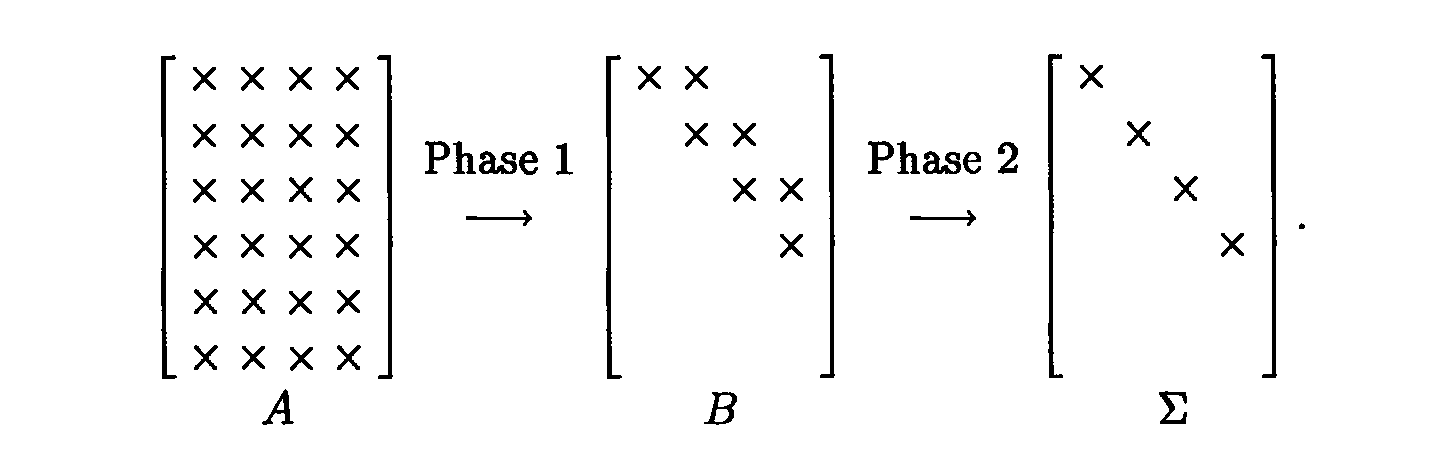
\includegraphics[width=0.94\textwidth]{../assets/figure-31-two-phases.png}
\parbox{0.94\textwidth}{\small 两阶段 SVD 计算的结构示意：第一阶段把稠密矩阵 $A$ 约化为双对角矩阵 $B$，第二阶段再把 $B$ 对角化为 $\Sigma$。}
\end{figure}

第一阶段需要有限次运算，成本为 $O(mn^2)$ 次浮点运算。第二阶段原则上需要
无限次运算，但标准算法超线性收敛，因此只需
$O(n\log|\log(\varepsilon_{\mathrm{machine}})|)$ 次迭代，就能达到
$\varepsilon_{\mathrm{machine}}$ 阶的精度（习题 25.2）。实际中通常把
$\varepsilon_{\mathrm{machine}}$ 当作常数，于是说收敛只需要 $O(n)$ 次迭代。
由于操作对象是双对角矩阵，每次迭代只需要 $O(n)$ 次浮点运算。因此，在只要求
奇异值而不要求奇异向量时，第二阶段总共需要 $O(n^2)$ 次浮点运算。也就是说，
尽管第一阶段是有限过程、第二阶段原则上是无限过程，但实际中后者的代价反而
小得多，这与对称特征值问题的情形相同。

\section*{Golub--Kahan 双对角化}

在 SVD 计算的第一阶段，通过在左侧和右侧施加不同的酉变换，把 $A$ 约化为
双对角形式。这一点不同于特征值计算：特征值算法必须在两侧施加相同的酉变换，
以保证每一步都是相似变换。在那里，我们只能在第一条次对角线以下引入零；而
在这里，矩阵可以完全三角化，并且还可以在第一条超对角线以上引入零。

最简单的实现方法是 Golub--Kahan 双对角化：在左侧和右侧交替使用 Householder
反射。每次左反射都会把主对角线以下的一列元素变成零；紧接着的右反射会把
第一条超对角线右侧的一行元素变成零，同时保留刚刚在该列中引入的零。对于
一个 $6\times4$ 矩阵，前两对反射的效果如下图所示。

\begin{figure}[H]
\centering
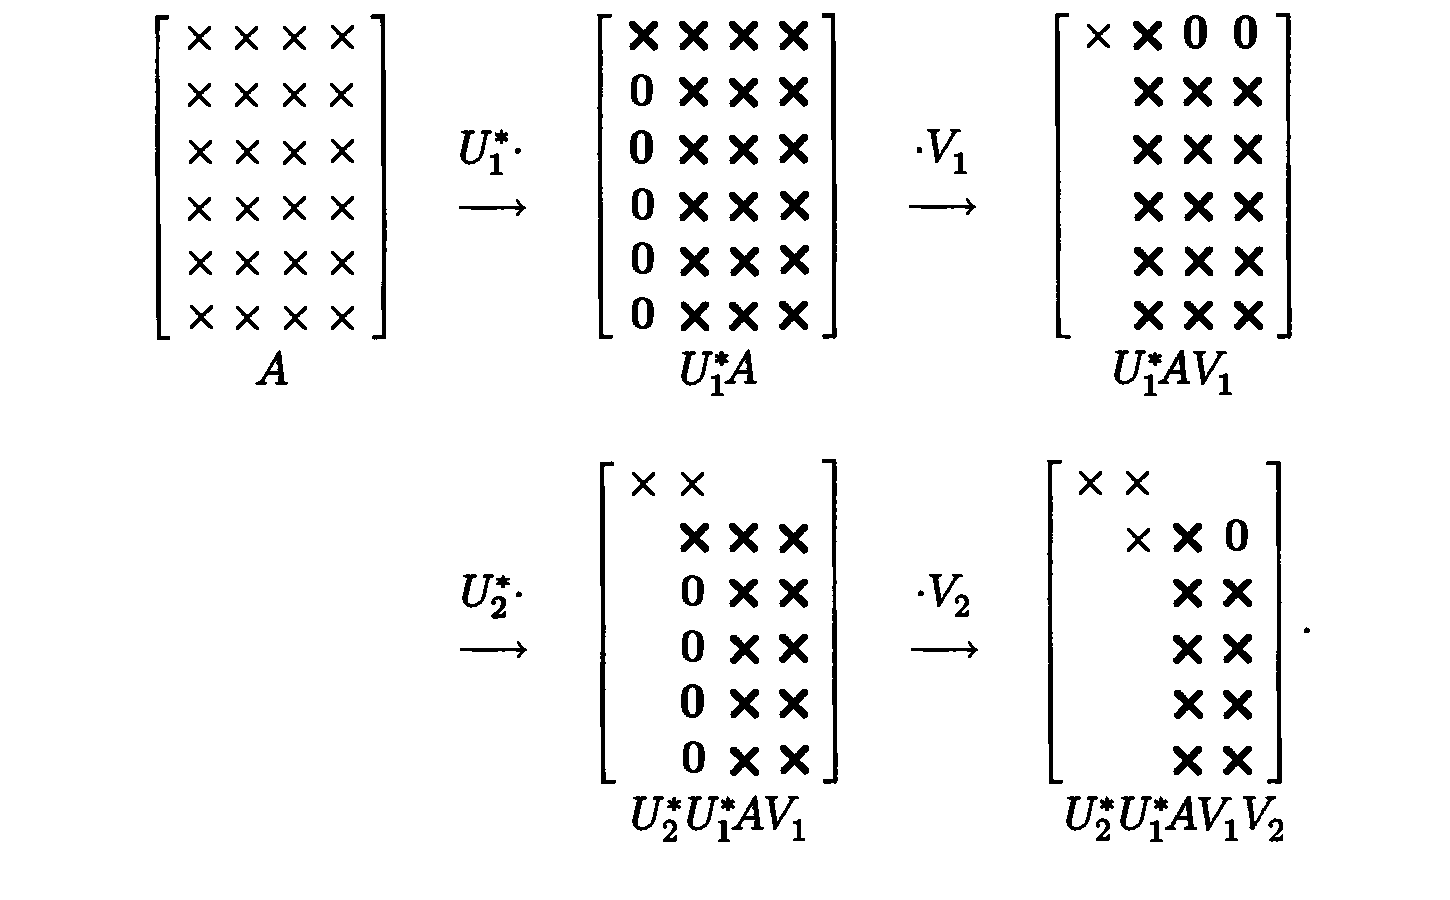
\includegraphics[width=0.96\textwidth]{../assets/figure-31-golub-kahan.png}
\parbox{0.96\textwidth}{\small Golub--Kahan 双对角化的前两对左右 Householder 反射：左乘 $U_1^*$、右乘 $V_1$，随后在剩余行列上重复这一过程。}
\end{figure}

左乘 $U_1^*$ 修改第 1 到第 $m$ 行，在第 1 列主对角线以下引入零。右乘
$V_1$ 修改第 2 到第 $n$ 列，在第 1 行引入零，同时不破坏第 1 列中已有的零。
接下来对第 2 到第 $m$ 行操作，再对第 3 到第 $n$ 列操作，如此继续。

整个过程结束时，左侧共施加了 $n$ 个反射，右侧施加了 $n-2$ 个反射。浮点
运算模式类似于两个交错进行的 Householder QR 分解：一个作用于 $m\times n$
矩阵 $A$，另一个作用于 $n\times m$ 矩阵 $A^*$。因此总运算量是 QR 分解
(10.9) 的两倍，即

\begin{equation}
\text{Golub--Kahan 双对角化的运算量：}\quad
\mathord{\sim}4mn^2-\frac{4}{3}n^3\quad\text{flops}.
\tag{31.4}
\end{equation}

\section*{第一阶段的更快方法}

当 $m\gg n$ 时，上面的运算量明显偏大。一次 QR 分解会在对角线以下的绝大
多数位置引入零，而 Golub--Kahan 方法的运算量却高出一倍。这一观察启发了另
一种双对角化方法：当 $m\gg n$ 时，先做 QR 分解。该方法最初由 Lawson 和
Hanson 提出，后来由 Chan 发展，称为 LHC 双对角化。

\begin{figure}[H]
\centering
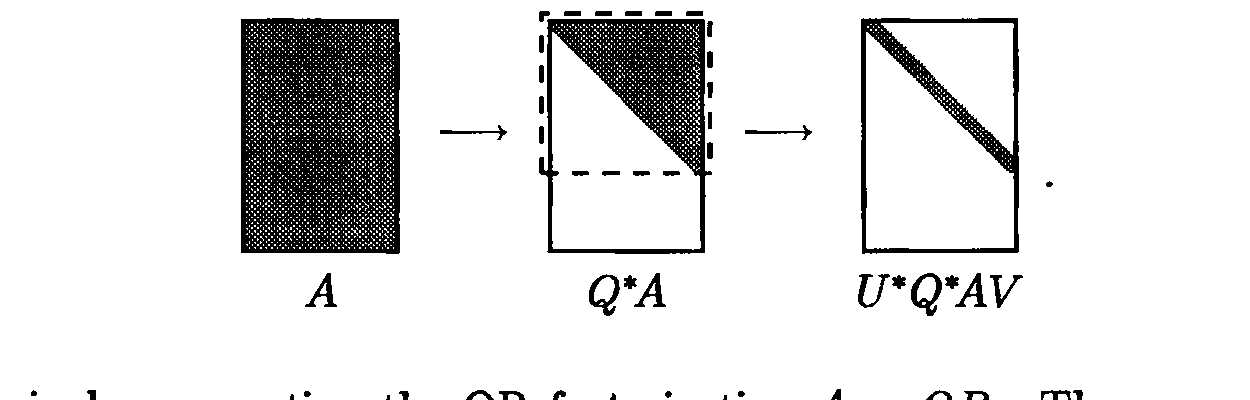
\includegraphics[width=0.90\textwidth]{../assets/figure-31-lhc.png}
\parbox{0.90\textwidth}{\small Lawson--Hanson--Chan 双对角化的结构示意：先通过 QR 分解得到 $Q^*A$，再对上方的方阵块作 Golub--Kahan 双对角化。}
\end{figure}

先计算 QR 分解 $A=QR$，再对 $R$ 作 Golub--Kahan 双对角化
$B=U^*RV$。QR 分解需要 $2mn^2-\frac{2}{3}n^3$ 次浮点运算，而此时
Golub--Kahan 过程只需作用于上方的 $n\times n$ 子矩阵，需要
$\frac{8}{3}n^3$ 次浮点运算。因此总运算量为

\begin{equation}
\text{LHC 双对角化的运算量：}\quad
\mathord{\sim}2mn^2+2n^3\quad\text{flops}.
\tag{31.5}
\end{equation}

当 $m>\frac53n$ 时，这个方法比 Golub--Kahan 双对角化更便宜（习题 31.1）。
有趣的是，LHC 过程先产生零，随后又在 $A$ 的上方 $n\times n$ 方块的下三角
部分破坏这些零，但总的运算量仍然减少了。

LHC 过程只有在 $m>\frac53n$ 时才有优势，但这个想法可以推广到任意 $m>n$
的情形。诀窍不是在计算开始时进行 QR 分解，而是在中间某个合适的时刻进行。
这是因为在 Golub--Kahan 过程中，$m>n$ 的矩阵会随着双对角化不断变得更“瘦”。
例如，初始长宽比为 $m/n=3/2$ 时，它会逐渐增长到 $5/3$、$2$ 乃至更大。
第 $k$ 步之后，剩余矩阵的长宽比为 $(m-k)/(n-k)$；当这个比值足够大时，
就适合进行 QR 分解，把问题化为一个方阵问题。

\begin{figure}[H]
\centering
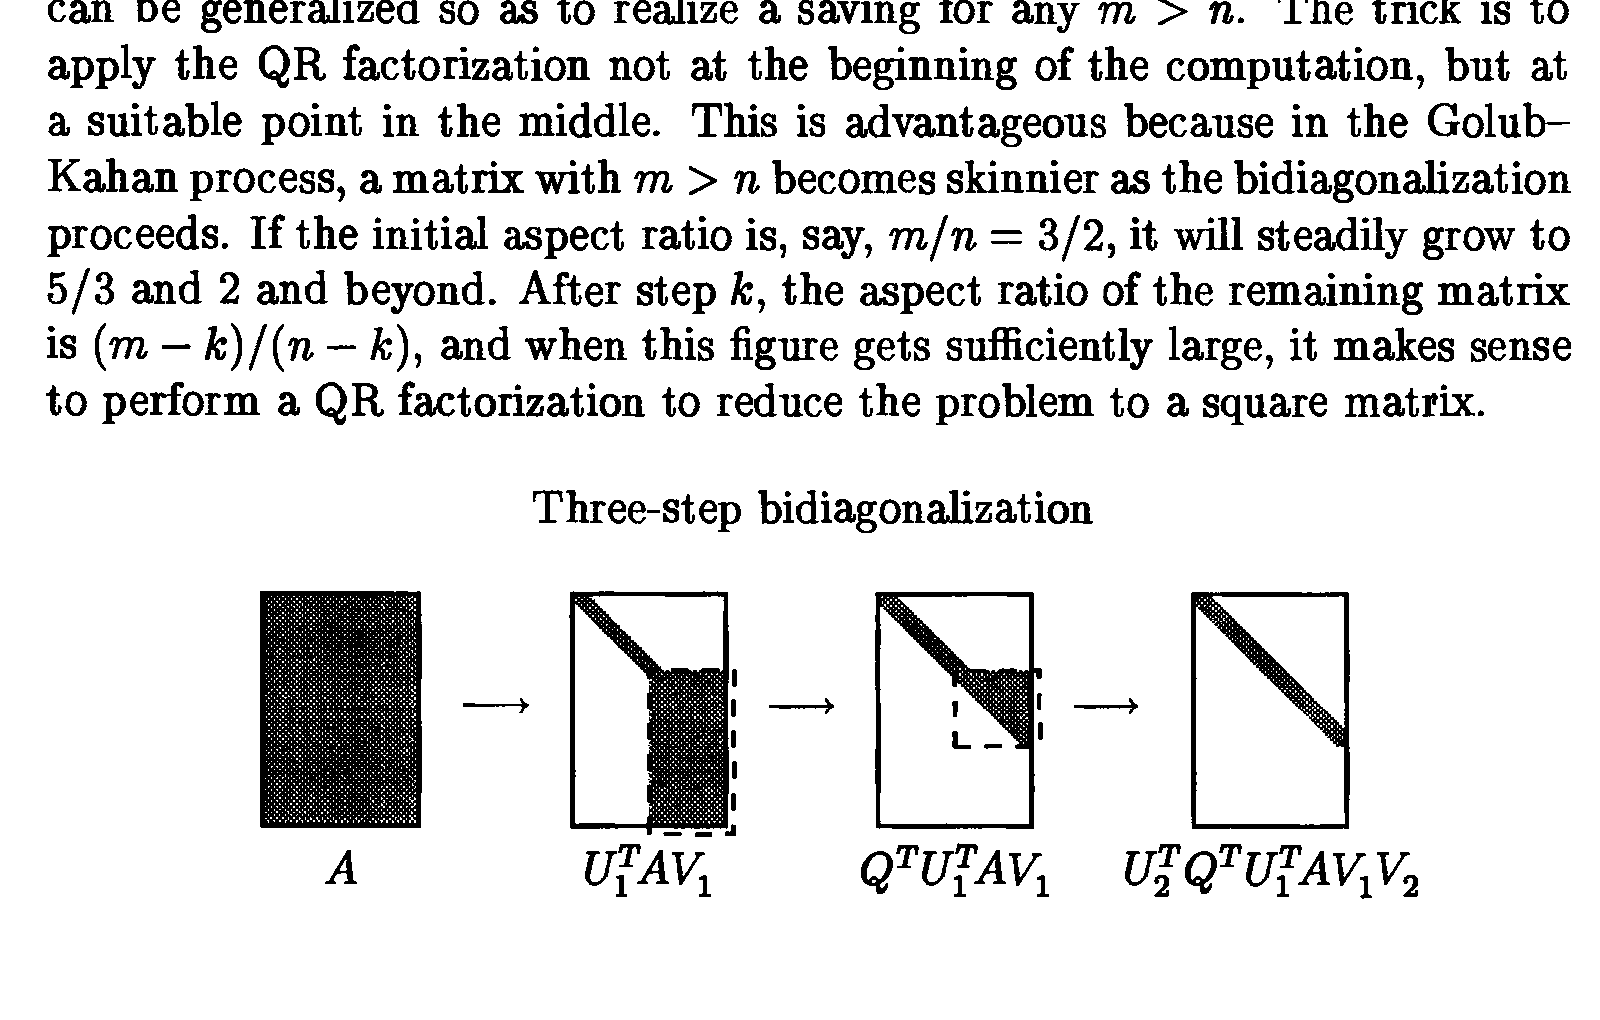
\includegraphics[width=0.98\textwidth]{../assets/figure-31-three-step.png}
\parbox{0.98\textwidth}{\small 三步双对角化的结构示意：在 Golub--Kahan 过程中途插入一次 QR 分解，再继续对剩余方阵块做双对角化。}
\end{figure}

什么时候应该进行 QR 分解？如果目标只是使运算量最小，答案很简单：当矩阵
达到长宽比

$$
\frac{m-k}{n-k}=2
$$

时（习题 31.2）。这一选择得到

\begin{equation}
\text{三步双对角化的运算量：}\quad
\mathord{\sim}4mn^2-\frac{4}{3}n^3-\frac{2}{3}(m-n)^3
\quad\text{flops}.
\tag{31.6}
\end{equation}

对于 $n<m<2n$，这比另外两种方法都有小幅改进。三种方法的运算量随
$m/n$ 的变化如图 31.1 所示。必须承认，三步方法的改进幅度很小，因此在真实
计算机上，除了运算量之外的其他因素也可能决定哪一种方法最好（见第 59 页）。

\begin{figure}[H]
\centering
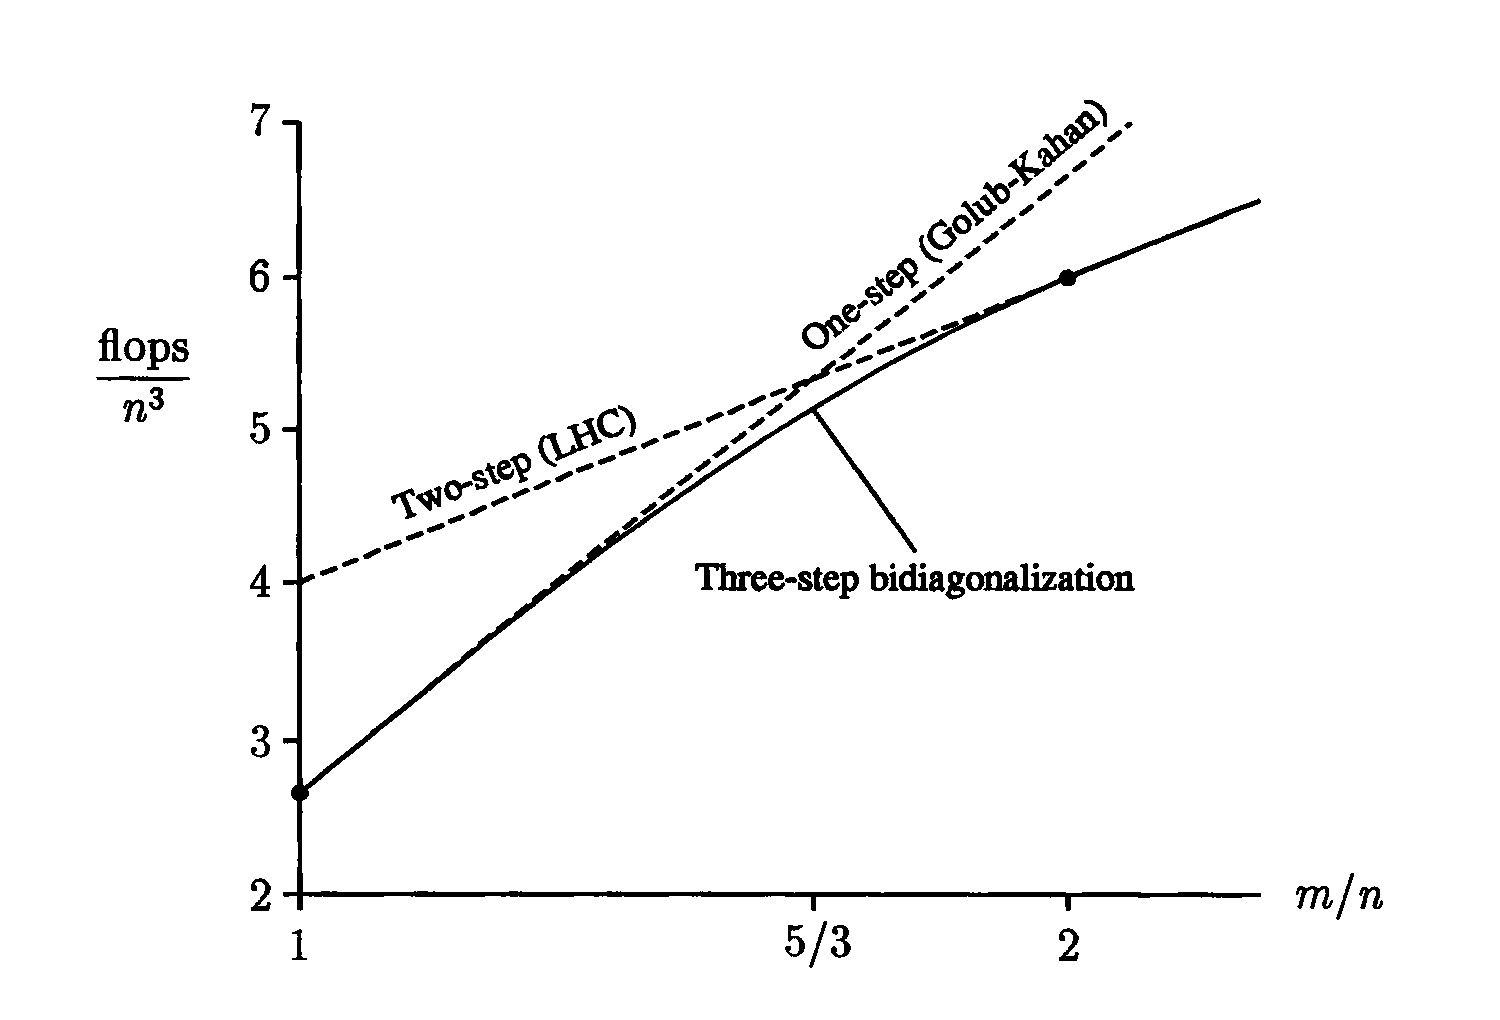
\includegraphics[width=0.92\textwidth]{../assets/figure-31-operation-count.png}
\parbox{0.92\textwidth}{\small 图 31.1. 对 $m\times n$ 矩阵应用三种双对角化算法时的运算量，分别由 (31.4)、(31.5)、(31.6) 给出。三步双对角化在另外两种方法之间提供了平滑的插值，但改进幅度并不大。}
\end{figure}

\section*{第二阶段}

在计算的第二阶段，需要求出双对角矩阵 $B$ 的 SVD。从 20 世纪 60 年代到
90 年代，标准算法是 QR 算法的一个变体。近些年，分治算法也变得具有竞争力；
未来它们很可能成为标准方法。这里不再给出细节。

\section*{习题}

\paragraph{31.1.}
(a) 证明：如正文所述且图 31.1 所示，LHC 双对角化开始优于 Golub--Kahan
双对角化的交叉长宽比为 $m/n=5/3$。

(b) 当 $m/n=5/3$ 时，三步双对角化比另外两种方法快多少比例？

\paragraph{31.2.}
证明：在三步双对角化中，执行 QR 分解的最优时刻，是矩阵达到长宽比 2 时。

\paragraph{31.3.}
证明：如果一个双对角矩阵的两条主对角线上的元素都非零，那么该矩阵的奇异值
互异。（参见习题 25.1。）

\paragraph{31.4.}
令 $A$ 为一个 $m\times m$ 上三角矩阵，主对角线上元素均为 0.1，对角线以上
所有元素均为 1。编写程序，用两种方法计算 $A$ 的最小奇异值：调用标准 SVD
软件；构造 $A^*A$ 并计算其最小特征值的平方根。令 $1\le m\le30$，在对数尺度
上把两种结果画成两条曲线。结果是否符合本讲关于这两种算法的一般讨论？

\paragraph{31.5.}
令 $A$ 为一个 $m\times n$ 矩阵，其元素是来自 $N(0,1)$ 的独立样本，其中
$N(0,1)$ 是均值为 0、方差为 1 的正态分布（参见习题 12.3）。令 $B$ 为如下
双对角矩阵：

$$
B=
\begin{bmatrix}
x_m&y_{n-1}&&&\\
&x_{m-1}&y_{n-2}&&\\
&&\ddots&\ddots&\\
&&&x_{m-(n-2)}&y_1\\
&&&&x_{m-(n-1)}
\end{bmatrix}.
$$

其中每个 $x$ 或 $y$ 都是一个独立 $\chi^2$ 分布样本的正平方根，其自由度等于
所附的下标。（自由度为 $k$ 的 $\chi^2$ 分布，就是 $k$ 个独立 $N(0,1)$
变量平方和的分布。）

(a) 证明：$A$ 与 $B$ 的奇异值分布相同。

(b) 通过实验验证这一结果。具体地，取 $m=100$、$n=50$，按上述方式构造
随机矩阵 $A$ 和 $B$，并把 $A$ 与 $B$ 的奇异值相互作图比较。

\end{document}
